\documentclass[12pt, letterpaper]{report}
\usepackage[utf8]{inputenc}
\usepackage[T1]{fontenc}
\usepackage[english,polish]{babel}
\usepackage{fancyhdr}
\usepackage{hyperref}
\usepackage{wrapfig}
\usepackage{subcaption}
\usepackage{graphicx}
\graphicspath{ {images/} }

\usepackage[margin=1.5cm]{geometry}

\title{
    Raport z postępów pracy \\
    \large Modelowanie elastycznych i nieelastycznych
    zderzeń obiektów\\
    metodą dynamiki molekularnej na potrzeby animacji
    komputerowych
}
\author{
    Kamil Pasterczyk \\
    \small Promotor: dr hab. inż. Tomasz Chwiej
}

\begin{document}

\maketitle
\tableofcontents

\chapter{Wstęp}
    \section{Opis}
    First document. This is a simple example, with no
    extra parameters or packages included. Hello world, nice to meet you

\chapter{Rozwinięcie}
    \section{Test poprawność działania algorytmów}
    \subsection{Opis testu}
    
    \begin{wrapfigure}{r}{0.5\textwidth}
        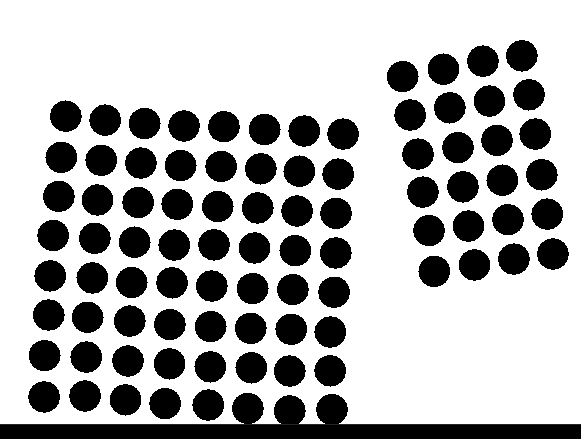
\includegraphics[width=0.9\linewidth]{objects_raw} 
        \caption{Widok aplikacji w fazie testów z widocznymi dwoma obiektami $8 \times 8$ oraz $6 \times 4$}
        \label{fig:wrapfig}
    \end{wrapfigure}
    Jeżeli wszystkie algorytmy symulujące odziaływania fizyczne zostały zimplementowane poprawnie 
    to w przypadku gdy nie występują żadne siły oporu energia całkowita układu powinna 
    być stała przez cały czas trwania symulacji. 
    Aby uzyskać poprawny obraz sytuacji należy uwzględnić
    wszystkie rodzaje energii w układzie: 
    \begin{enumerate}
        \item Energia potencjalna grawitacji
        \item Energia kinetyczna
        \item Energia potencjalna węwnątrz obiektu
        \item Energia potencjalna odpychająca pomiędzy obiektami a podłożem
        \item Energia potencjalna odpychająca pomiędzy dwoma obiektami
    \end{enumerate}
    Do testu zachowania energii wykorzystane są 
    dwa obiekty o rozmiarach odpowiednio $8 \times 8$ i $6 \times 4$ oraz statyczne podłoże. Obiekty
    znajdują się w polu grawitacyjnym, nie ma żadnych sił oporu/tarcia.

    \subsubsection{Parametry symulacji}
    $g = 9.81 [\frac{m}{s^2}]$\\
    $dt = 10^{-5} [s]$\\
    $t_{max} = 8 [s]$\\ \\ \\ \\

    \pagebreak
    \subsection{Wyniki}
    \begin{figure}[h]
        \centering
        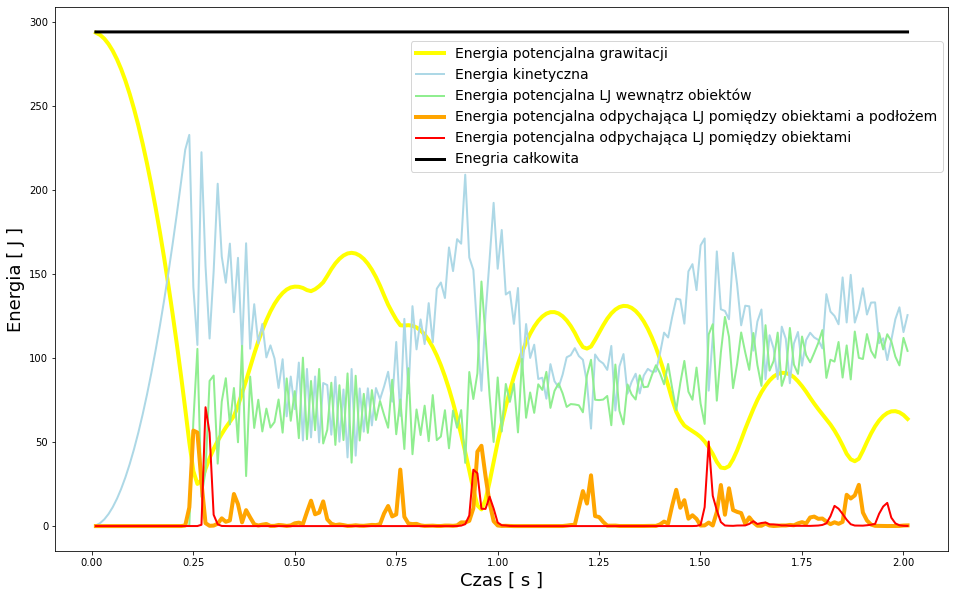
\includegraphics[width=13cm]{energy_test_0to2s}
        \caption{Zmiana enegii w czasie dla układu w ciągu pierwszych 2 sekund}
    \end{figure}

    Przy zderzeniach pomiędzy obiektami oraz pomiędzy obiektem i podłożem energia potencjalna
    odpychająca Lennarda-Jonesa oznaczona kolejno kolorami pomarańczowym i czerwonym
    wyraźnie wzrasta.
    \begin{figure}[h]
        \centering
        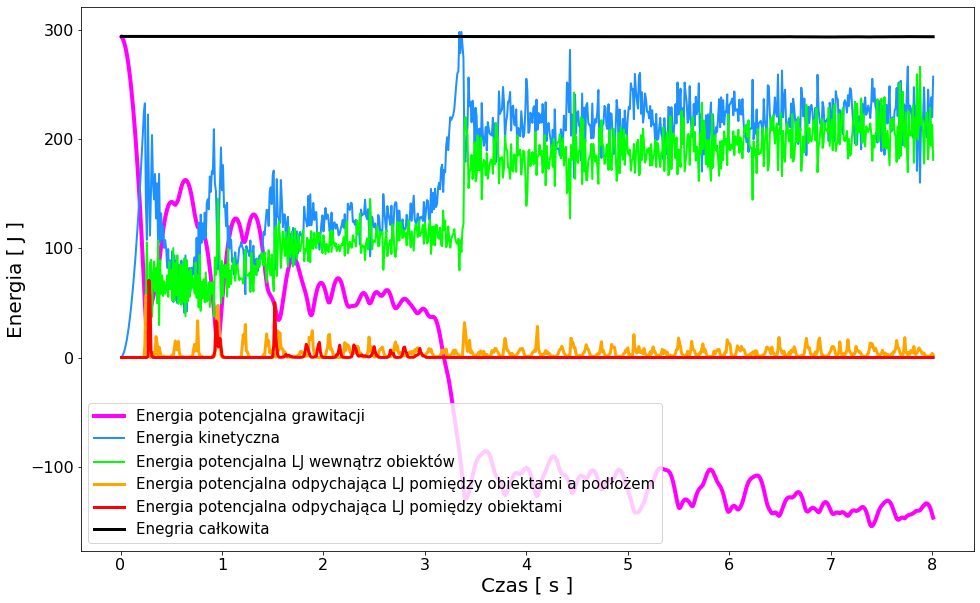
\includegraphics[width=13cm]{energy_test_0to8s}
        \caption{Zmiana enegii w czasie dla układu w ciągu pierwszych 8 sekund}
    \end{figure}
    
    Po upłynięciu kilku sekund obiekty zostają przy podłożu, energia będąca początkowo energią
    potencjalną grawitacji została w większości zamieniona na energię kinetyczną oraz energię
    wewnętrzną. Obiekty nie odbijają się one już między sobą.
    Zmiana energii całkowitej w czasie działania całej symulacji była mniejsza niż $1\%$. Na tej
    podstawie można uznać, że algorytmy zostały zaimplementowane poprawnie.


    \section{Test wydajności dla dwóch algorytmów obsługi zderzeń między obiektami}
    \subsection{Opis algorytmów}
    Naszym celem jest obliczanie siły poędzy odpowiednimi węzłami w taki sposób aby 
    obiekty przy zderzeniu odpychały się od siebie.
    
    \begin{figure}[h]

        \begin{subfigure}{0.5\textwidth}
        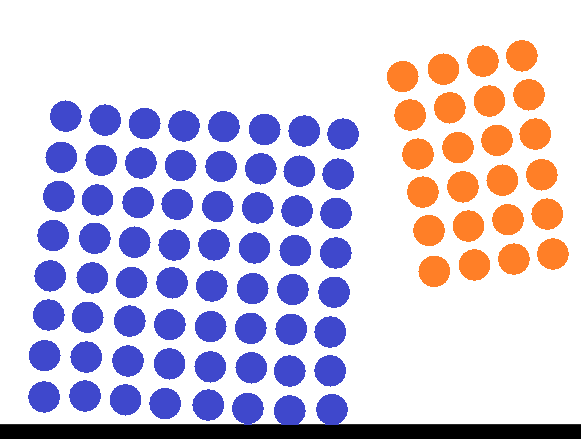
\includegraphics[width=0.9\linewidth, height=6cm]{objects_unoptimized} 
        \caption{Metoda "każdy z każdym"}
        \label{fig:subim1}
        \end{subfigure}
        \begin{subfigure}{0.5\textwidth}
        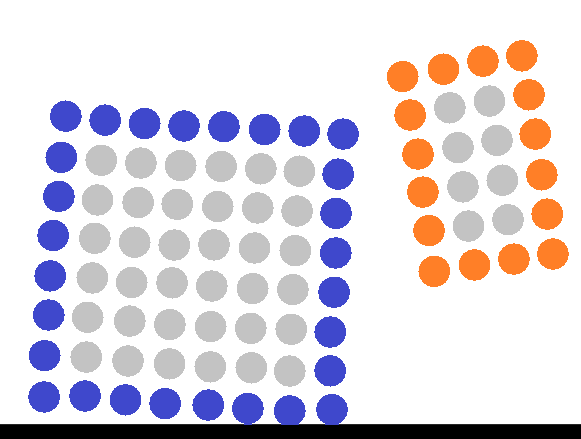
\includegraphics[width=0.9\linewidth, height=6cm]{objects_optimized}
        \caption{Metoda węzłów granicznych}
        \label{fig:subim2}
        \end{subfigure}
        
        \caption{Reprezentacja dwóch metod obsługi zderzeń}
        \label{fig:image2}
    \end{figure}

    Dla metody (a) oddziaływanie liczone jest pomiędzy każdym węzłem o kolorze 
    niebieskim z każdym węzłem o
    kolorze pomarańczowym. Metoda o złożoności $O(n^2)$ gdzie $n$ to liczba węzłów.
    Jest to metoda bardzo wolna, lecz dająca poprawne rezultaty w każdym symulowanym przypadku.\\

    Dla metody (b) oddziaływanie ponownie liczone jest pomiędzy każdym węzłem o kolorze niebieskim z każdym
    węzłem o kolorze pomarańczowym, tym razem jednak oznaczone są jedynie węzły brzegowe.
    Metoda ta jest szczególnie efektywna dla obiektów kwadratowych o boku $n$, gdzie z $n^2$
    rozpatrywanych węzłów ta liczba jest zmniejszona do zaledwie $4(n-1)$ węzłów.
    Należy zwrócić uwagę, że metoda ta nie będzie poprawnie odwzorowywać oddziaływań dla
    obiektów zagnieżdżonych w sobie. Przykładowa sytuacja, w której algorytm nie zadziała poprawnie
    to symulacja penetracji obiektu przy kuli/naboju.

    \begin{center}
        \begin{tabular}{||c c c c||} 
         \hline
         węzły w boku obiektu & $iteracje / [s]$ dla (a) & $iteracje / [s]$ dla (b) & krotność przyśpieszenia \\ [0.5ex] 
         \hline\hline
         3 & 6 & 87837 & 787 \\ 
         \hline
         5 & 7 & 78 & 5415 \\
         \hline
         9 & 545 & 778 & 7507 \\
         \hline
         15 & 88 & 788 & 6344 \\
         \hline
         21 & 88 & 788 & 6344 \\
         \hline
         25 & 88 & 788 & 6344 \\
         \hline
         30 & 88 & 788 & 6344 \\
         \hline
         35 & 88 & 788 & 6344 \\
         \hline
         40 & 88 & 788 & 6344 \\ 
         \hline
         45 & 88 & 788 & 6344 \\ 
         \hline
         50 & 88 & 788 & 6344 \\
         \hline
         55 & 88 & 788 & 6344 \\ 
         \hline
         60 & 88 & 788 & 6344 \\ [1ex] 
         \hline
        \end{tabular}
    \end{center}

\chapter{Zakończenie}
    \section{Dodatek}

    \subsection{Filmik prezentujące działanie aplikacji}

    \subsubsection{Przekazanie energii między dwoma sztywnimi obiektami}

    Mniejszy obiekt $3 \times 3$ po odbiciu od większego obiektu $8 \times  8$ znajdującego się pod nim wznosi się na
    wysokość o wiele większą, niż ta z której rozpoczął spadek swobodny.
    Występuje tutaj przekazanie części energii z obiektu większego do mniejszego - sama zasada energii jest zachowana.

    \paragraph{
        \url{https://youtu.be/nolLh6CSa-8}
    }

    \subsubsection{Przekazanie energii między dwoma miękkimi obiektami}
    W tym przypadku obiekty są mniej sztywne,
    obiekt $3 \times 3$ po odbiciu od obiektu $8 \times  8$ wznosi się na wyraźnie mniejszą wysokość niż w przypadku bardziej sztywnych obiektów
    (jednak wciąż wyżej niż punkt z którego zaczął spadać). Można to wytłumaczyć tym,
    że znaczna część energii która w poprzednim przypadku była częścią ruchu postępowego,
    teraz stała się energią wewnętrzną obiektów (wibracje obiektów pochłaniają część energii).

    \paragraph{
        \url{https://youtu.be/q2uYx8uLl3w}
    }

    \subsubsection{Proste zderzenie dwóch obiektów}
    \paragraph{
        \url{https://www.youtube.com/watch?v=4cGcL_5yUt4}
    }

    \subsection{Repozytorium}
    Repozytorium z kodem projektu znajduje się pod adresem:
    \paragraph{
        \url{https://github.com/theYiome/elastic-objects-rs}
}

\end{document}